\subsection{PostgreSQL}

\begin{frame}
 \frametitle{Diagram encji}
 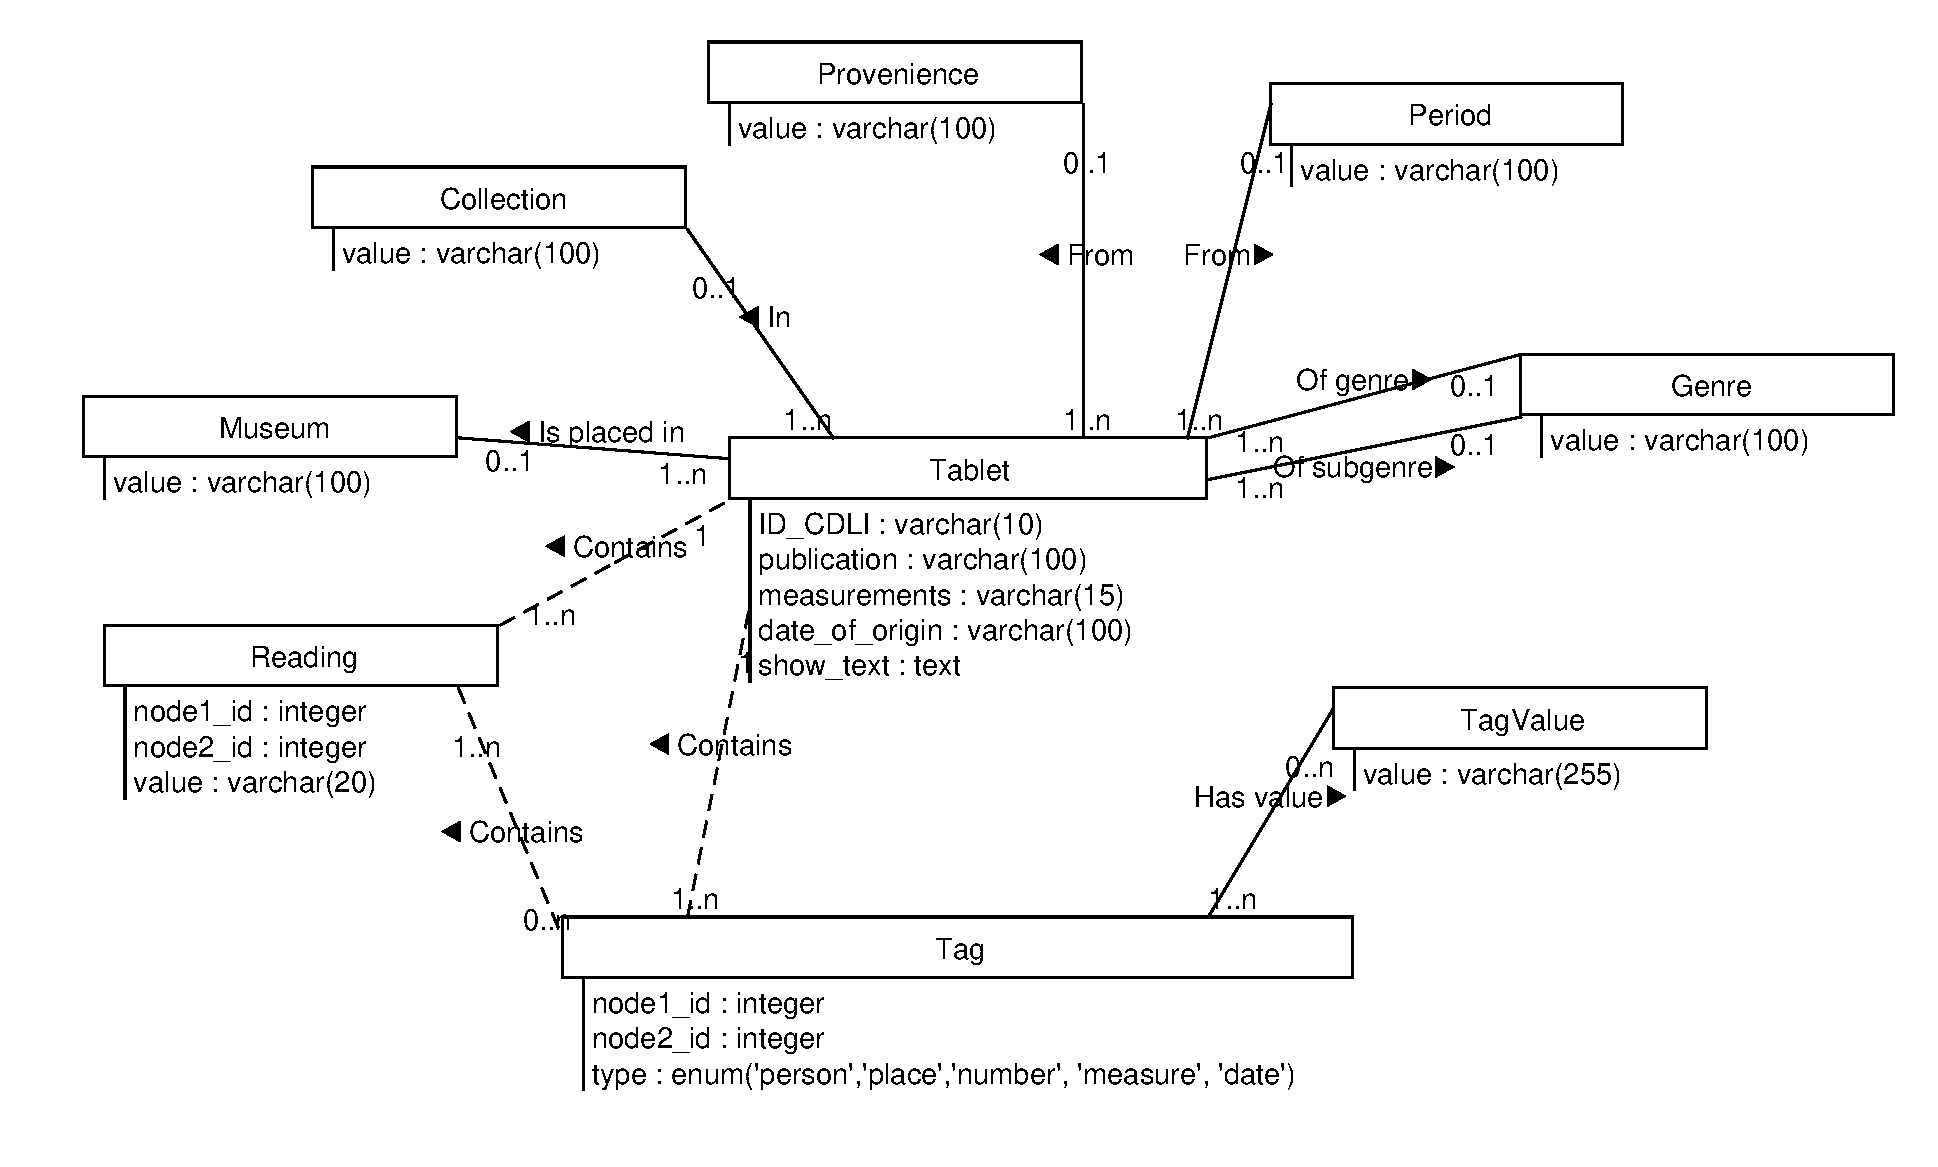
\includegraphics[width=100mm]{../diagramy/diagram-encji-maly.pdf}
\end{frame}

\begin{frame}
 \frametitle{Tłumaczenie zapytań: inicjalizacja}
 \begin{block}{Select}
SELECT t.id, t.id\_cdli, t.publication, t.measurements, t.origin\_date, \\
~~~~~~~p.value as provenience, pd.value as period, \\
~~~~~~~g1.value as genre, g2.value as subgenre, \\
~~~~~~~c.value as collection, t.text 
 \end{block}
\begin{block}{From}
FROM tablet t \\
~~LEFT JOIN provenience p ON p.id=t.provenience\_id \\
~~LEFT JOIN collection c ON c.id=t.collection\_id \\
~~LEFT JOIN genre g1 ON g1.id=t.genre\_id \\
~~LEFT JOIN genre g2 ON g2.id = t.subgenre\_id \\
~~LEFT JOIN period pd ON pd.id = t.period\_id \\
\end{block}

\end{frame}

\begin{frame}
 \frametitle{Tłumaczenie zapytań: zapytania proste}
\begin{block}{provenience: wartosc}
p.value LIKE 'wartosc'
\end{block}

\begin{block}{publication: wartosc}
t.publication LIKE ’wartosc’
\end{block}

\begin{block}{period: wartosc}
pd.value LIKE 'wartosc'
\end{block}

\begin{block}{genre: wartosc}
g1.value LIKE 'wartosc' OR g2.value LIKE 'wartosc'
\end{block}

\begin{block}{cdli\_id: wartosc}
 t.cdli\_id LIKE 'wartosc'
\end{block}


\end{frame}

\begin{frame}
 \frametitle{Tłumaczenie zapytań: treść tabliczki}

% \begin{block}{From}
% 
% INNER JOIN ( \\
% 
% ) AS sequence ON sequence.id\_tab = t.id \\
%  \end{block}

 \begin{block}{Zapytanie o treść tablczki}
\begin{scriptsize}
SELECT \\
~~id\_tab, \\
~~CAST(array\_accum(nodes) as TEXT) as nodes,\\
~~$<$id\_seq$>$ AS id\_seq\\
FROM (\\
~~SELECT\\
~~~~t1.node1\_id \% 1000000 AS id\_tab,\\
~~~~’\{’ $||$ t1.node1\_id $||$ ’,’ $||$ t$<$dl\_sekw$>$.node2\_id $||$ ’\}’ AS nodes,\\
~~~~1 AS id\_seq\\
~~FROM\\
~~~~readings t1\\
~~~~LEFT JOIN readings t2 ON (t2.node1 = t1.node2)\\
~~~~LEFT JOIN $<$nazwa\_tabeli$>$ t3 ON (t3.node1 = t2.node2)\\
~~~~...\\
~~~~LEFT JOIN $<$nazwa\_tabeli$>$ t$<$dl\_sekw$>$ ON (t$<$dl\_sekw$>$.node1 = t$<$dl\_sekw-1$>$.node2)\\
~~WHERE\\
~~~~t1.value LIKE ’$<$sekw[1]$>$’\\
~~~AND\\
~~~~t2.value LIKE ’$<$sekw[2]$>$’\\
% ~~~AND\\
% ~~~~t3.value LIKE ’$<$sekw[3]$>$’\\
% ~~~AND\\
~~~~...\\
~~~AND\\
~~~~t$<$dl\_sekw$>$.value LIKE ’$<$sekw[$<$dl\_sekw$>$]$>$’\\
) AS a
GROUP BY id\_tab

\end{scriptsize}
 \end{block}

\end{frame}

\begin{frame}
 \frametitle{Tłumaczenie zapytań: operatory}
\begin{block}{/ -- or}
SELECT \\
~~id\_tab, \\
~~CAST(array\_accum(nodes) as TEXT) as nodes, \\
~~$<$id\_sekw$>$ as id\_seq\\
FROM \\
(\\
~~$<$zapytanie1$>$\\
~~\textbf{UNION}\\
~~$<$zapytanie2$>$\\
)\\
as c\\
GROUP BY id\_tab
\end{block}

\end{frame}


\begin{frame}
 \frametitle{Tłumaczenie zapytań: operatory}
\begin{block}{+ -- and}
SELECT id\_tab, \\
~~~~~~ CAST(array\_accum(nodes) as TEXT) as nodes, \\
~~~~~~ $<$id\_sekw$>$ as id\_seq\\
FROM\\
(\\
~~$<$zapytanie1$>$\\
~~UNION\\
~~$<$zapytanie2$>$\\
) as c \\
GROUP BY id\_tab\\
\textbf{HAVING COUNT(DISTINCT id\_seq)=2} \\


\end{block}
\end{frame}

\begin{frame}
 \frametitle{Tłumaczenie zapytań: operatory}
\begin{block}{$--$ -- not}
SELECT \\
~~id\_tab, \\
~~'' as nodes, \\
~~$<$id\_sekw$>$ as id\_seq\\
FROM\\
(\\
~~(SELECT id as id\_tab from tablet)\\
~~~~\textbf{EXCEPT}\\
~~(SELECT id\_tab from\\
~~~~$<$zapytanie\_negowane$>$ as a\\
~~)   \\
) as b
\end{block}

\end{frame}
